\documentclass[12pt]{article}
\usepackage[utf8]{inputenc, }
\usepackage{graphicx}
\usepackage{hyperref}
\usepackage[margin=1in]{geometry}
\usepackage{setspace}
\usepackage{color}
\usepackage{pdfpages}
\usepackage{amsmath}
\usepackage{amsfonts}
\usepackage{float}
\usepackage{tikz}
\usepackage{pgfplots}
\usepackage{enumitem}
\usepackage{xpatch}
\usepackage{svg}
\usepackage{mathrsfs}
\usepackage{steinmetz}
\usepackage{tikz}
\usetikzlibrary{shapes.misc}
\usetikzlibrary{patterns}
% \usepackage[nocheck]{fancyhdr}

\sloppy
\definecolor{lightgray}{gray}{0.5}
\setlength{\parindent}{0pt}

\hypersetup{
    colorlinks,
    citecolor=black,
    filecolor=black,
    linkcolor=black,
    urlcolor=black
    pdftitle={EE300 İsmail Enes Bülbül}
}
\onehalfspacing

% \raggedright

\title{EE301 Homework-4}
\author{İsmail Enes Bülbül, Eren Meydanlı, Ahmet Caner Akar}
%\date{October 2022}
\renewcommand*\contentsname{Table of Contents}
\renewcommand*{\refname}{}
% \fancyhf{} % sets both header and footer to nothing
% \renewcommand{\headrulewidth}{0pt}
\begin{document}

\maketitle
% \tableofcontents
% \newpage

    \section*{Question 1}
    \subsection*{a)}
    \begin{math} 
    x_s(t) = x(t) s(t) = \displaystyle\sum_{n=-\infty}^{\infty} x(t) \delta(t-nT_s) = \displaystyle\sum_{n=-\infty}^{\infty} x(nT_s) \delta(t-nT_s)\\ 
    \textrm{where } T_s \textrm{ is called the sampling period.}\\
    \textrm{By the modulation property of CTFT: } X_s(j\omega) = \frac{1}{2\pi} X(j\omega)*S(j\omega) \\ \\
    \textrm{s(t) is a periodic signal, therefore we should first find its CTFS representation: }\\
    s(t) = \displaystyle\sum_{k=-\infty}^{\infty} a_k e^{jk\omega_s t}, \omega_s = \frac{2\pi}{T_s} \\
    a_k = \frac{1}{T_s} \displaystyle\int_{-T_s/2}^{T_s/2} \underbrace{s(t)}_{\delta(t)} e^{-jk\omega_s t} dt \Rightarrow a_k = \frac{1}{T_s} \\
    s(t) = \displaystyle\sum_{k=-\infty}^{\infty} \frac{1}{T_s} e^{jk\omega_s t} \longrightarrow S(j\omega) = \displaystyle\sum_{k=-\infty}^{\infty} \frac{2\pi}{T_s} \delta(\omega-k\omega_s) \\ \\
    X_s(j\omega) = \frac{1}{2\pi} X(j\omega)*\displaystyle\sum_{k=-\infty}^{\infty} \frac{2\pi}{T_s} \delta(\omega-k\omega_s) = \displaystyle\sum_{k=-\infty}^{\infty} \frac{1}{T_s} X(j(\omega-k\omega_s)) 
    \end{math} \\ \\
    From the Nyquist sampling theorem, the inequality \(\omega_s \geq 2\Delta\omega\) should be satisfied so that the shifted replicas of \(X(j\omega)\) do not overlap. Thus, it yields perfect reconstruction of the signal \(x(t)\) from \(x_s(t)\) with no aliasing. So, the minumum sampling rate, \(\omega_s = 2\Delta\omega\). The Fourier transform of the sampling system output, \(X_s(j\omega)\) can be seen below. \\ 
     \begin{center}
  \begin{tikzpicture}
\begin{axis}[
    axis lines = middle,
    scale only axis,
    width=12cm, 
    height=6cm,
    ymin = -0.2,
    ymax = 0.8,
    xlabel = \(\omega\),
    xlabel style={xshift=0.4cm},
    ylabel style={yshift=0.4cm},
    ylabel = {\(X_s(j\omega)\)},
    xtick={-3*pi, -2*pi, -1*pi, 0, 1*pi, 2*pi, 3*pi},
    xticklabel style={font=\footnotesize,fill=white,inner sep=2pt},
    xticklabels={$-3\Delta\omega$,$-2\Delta\omega$,$-\Delta\omega$,,$\Delta\omega$,$2\Delta\omega$,$3\Delta\omega$},
    samples=500,
    enlargelimits=true,
    ytick style={draw=none},
    yticklabels={draw=none},
    ]
       \addplot [domain=-1*pi:0,style=very thick,black] {(x+pi)/(2*pi)};
       \addplot [domain=0:1*pi,style=very thick,black] {(pi-x)/(2*pi)};
       \addplot [domain=-2*pi:-1*pi,style=very thick,black] {-(x+pi)/(2*pi)};
       \addplot [domain=-3*pi:-2*pi,style=very thick,black] {(x+3*pi)/(2*pi)};
       \addplot [domain=1*pi:2*pi,style=very thick,black] {(x-pi)/(2*pi)};
       \addplot [domain=2*pi:3*pi,style=very thick,black] {-(x-3*pi)/(2*pi)};
       \filldraw[black] (axis cs: 10,0.3) circle (1.2pt) node[anchor=west]{};
        \filldraw[black] (axis cs: 10.5,0.3) circle (1.2pt) node[anchor=west]{};
        \filldraw[black] (axis cs: 11,0.3) circle (1.2pt) node[anchor=west]{};
        \filldraw[black] (axis cs: -10,0.3) circle (1.2pt) node[anchor=west]{};
        \filldraw[black] (axis cs: -10.5,0.3) circle (1.2pt) node[anchor=west]{};
        \filldraw[black] (axis cs: -11,0.3) circle (1.2pt) node[anchor=west]{};
        \draw[dashed] (axis cs: 2*pi,0)--(axis cs: 2*pi,0.5);
        \draw[dashed] (axis cs: -2*pi,0)--(axis cs: -2*pi,0.5);
        
\end{axis}
\end{tikzpicture}
\end{center}
    
    \subsection*{b)}
    \(X(j\omega)\) is not symmetric with respect to y-axis, thus from the symmetry property of CTFT it can be concluded that \(x(t)\) is a complex-valued signal. 
    \subsubsection*{i)}
    Since the sampling rate of the signal is equal to the Nyquist rate, the aliasing does not occur. The Fourier transform of \(X_s(j\omega)\) is plotted below for \( T_s = \frac{\pi}{\Delta\omega}\). 
         \begin{center}
  \begin{tikzpicture}
\begin{axis}[
    axis lines = middle,
    scale only axis,
    width=12cm, 
    height=6cm,
    ymin = -0.2,
    ymax = 0.8,
    xlabel = \(\omega\),
    xlabel style={xshift=0.4cm},
    ylabel style={yshift=0.4cm},
    ylabel = {\(X_s(j\omega)\)},
    xtick={-4*pi,-3*pi, -2*pi, -1*pi, 0, 1*pi, 2*pi, 3*pi},
    xticklabel style={font=\footnotesize,fill=white,inner sep=2pt},
    xticklabels={$-4\Delta\omega$,$-3\Delta\omega$,$-2\Delta\omega$,$-\Delta\omega$,,$\Delta\omega$,$2\Delta\omega$,$3\Delta\omega$},
    samples=500,
    enlargelimits=true,
    ytick style={draw=none},
    yticklabels={draw=none},
    ]
       \addplot [domain=0:1*pi,style=very thick,black] {(pi-x)/(2*pi)};
       \addplot [domain=-2*pi:-pi,style=very thick,black] {-(x+pi)/(2*pi)};
       \addplot [domain=2*pi:3*pi,style=very thick,black] {-(x-3*pi)/(2*pi)};
       \addplot [domain=-4*pi:-3*pi,style=very thick,black] {-(x+3*pi)/(2*pi)};
       \filldraw[black] (axis cs: 10,0.3) circle (1.2pt) node[anchor=west]{};
        \filldraw[black] (axis cs: 10.5,0.3) circle (1.2pt) node[anchor=west]{};
        \filldraw[black] (axis cs: 11,0.3) circle (1.2pt) node[anchor=west]{};
        \filldraw[black] (axis cs: -13.1,0.3) circle (1.2pt) node[anchor=west]{};
        \filldraw[black] (axis cs: -13.6,0.3) circle (1.2pt) node[anchor=west]{};
        \filldraw[black] (axis cs: -14.1,0.3) circle (1.2pt) node[anchor=west]{};
        \draw[very thick] (axis cs: -2*pi,0)--(axis cs: -2*pi,0.5);
        \draw[very thick] (axis cs: -4*pi,0)--(axis cs: -4*pi,0.5);
        \draw[very thick] (axis cs: 0,0)--(axis cs: 0,0.5);
        \draw[very thick] (axis cs: 2*pi,0)--(axis cs: 2*pi,0.5);
\end{axis}
\end{tikzpicture}
\end{center}
    \subsubsection*{ii)}
    As it can be seen from the graph of the Fourier transform of \(x(t)\), the graph is not symmetric with respect to y-axis, i.e., \(X(j\omega)\) has no component at negative frequencies. Therefore, as it can be seen from the graph of \(X_s(j\omega)\) below, the aliasing can be avoided even when \(T_s = \frac{2\pi}{\Delta\omega}\) which below the Nyquist rate. 
   \begin{center}
  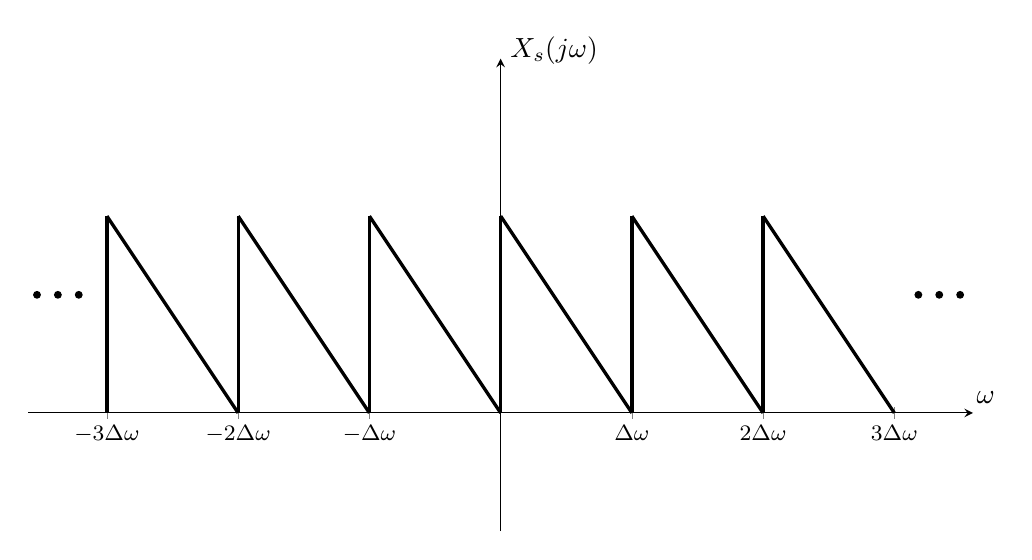
\begin{tikzpicture}
\begin{axis}[
    axis lines = middle,
    scale only axis,
    width=12cm, 
    height=6cm,
    ymin = -0.2,
    ymax = 0.8,
    xlabel = \(\omega\),
    xlabel style={xshift=0.4cm},
    ylabel style={yshift=0.4cm},
    ylabel = {\(X_s(j\omega)\)},
    xtick={-3*pi, -2*pi, -1*pi, 0, 1*pi, 2*pi, 3*pi},
    xticklabel style={font=\footnotesize,fill=white,inner sep=2pt},
    xticklabels={$-3\Delta\omega$,$-2\Delta\omega$,$-\Delta\omega$,,$\Delta\omega$,$2\Delta\omega$,$3\Delta\omega$},
    samples=500,
    enlargelimits=true,
    ytick style={draw=none},
    yticklabels={draw=none},
    ]
       \addplot [domain=0:1*pi,style=very thick,black] {(pi-x)/(2*pi)};
       \addplot [domain=pi:2*pi,style=very thick,black] {-(x-2*pi)/(2*pi)};
       \addplot [domain=-pi:0,style=very thick,black] {(-x)/(2*pi)};
       \addplot [domain=-2*pi:-pi,style=very thick,black] {-(x+pi)/(2*pi)};
       \addplot [domain=-3*pi:-2*pi,style=very thick,black] {-(x+2*pi)/(2*pi)};
       \addplot [domain=2*pi:3*pi,style=very thick,black] {-(x-3*pi)/(2*pi)};
       \filldraw[black] (axis cs: 10,0.3) circle (1.2pt) node[anchor=west]{};
        \filldraw[black] (axis cs: 10.5,0.3) circle (1.2pt) node[anchor=west]{};
        \filldraw[black] (axis cs: 11,0.3) circle (1.2pt) node[anchor=west]{};
        \filldraw[black] (axis cs: -10.1,0.3) circle (1.2pt) node[anchor=west]{};
        \filldraw[black] (axis cs: -10.6,0.3) circle (1.2pt) node[anchor=west]{};
        \filldraw[black] (axis cs: -11.1,0.3) circle (1.2pt) node[anchor=west]{};
        \draw[very thick] (axis cs: -2*pi,0)--(axis cs: -2*pi,0.5);
        \draw[very thick] (axis cs: -3*pi,0)--(axis cs: -3*pi,0.5);
        \draw[very thick] (axis cs: -pi,0)--(axis cs: -pi,0.5);
        \draw[very thick] (axis cs: pi,0)--(axis cs: pi,0.5);
        \draw[very thick] (axis cs: 0,0)--(axis cs: 0,0.5);
        \draw[very thick] (axis cs: 2*pi,0)--(axis cs: 2*pi,0.5);
\end{axis}
\end{tikzpicture}
\end{center}

    \subsection*{c)}
    The minimum sampling period, \(T_s = \frac{\pi}{2\Delta\omega} \Rightarrow\) minimum sampling rate, \( \frac{1}{T_s} = \frac{2\Delta\omega}{\pi}\). The Fourier transform of \(X_s(j\omega)\) can be seen below. Also, the corresponding time-domain signal is band-pass as it can be seen from the graph of its Fourier transform. 
    \begin{center}
  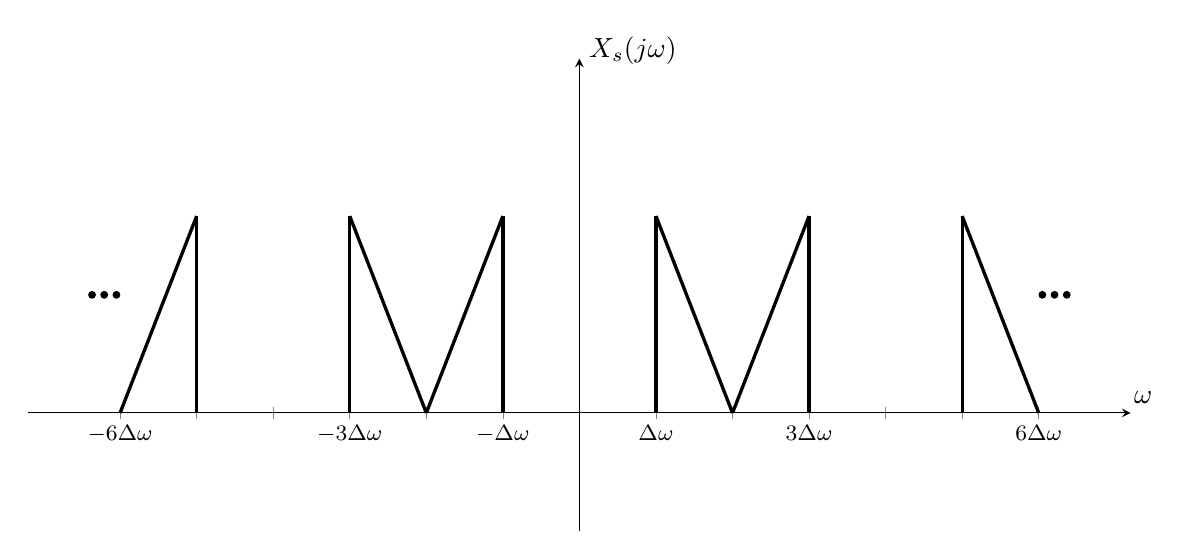
\begin{tikzpicture}
\begin{axis}[
    axis lines = middle,
    scale only axis,
    width=14cm, 
    height=6cm,
    ymin = -0.2,
    ymax = 0.8,
    xlabel = \(\omega\),
    xlabel style={xshift=0.4cm},
    ylabel style={yshift=0.4cm},
    ylabel = {\(X_s(j\omega)\)},
    xtick={-6*pi, -5*pi, -4*pi, -3*pi, -2*pi, -1*pi, 0, 1*pi, 2*pi, 3*pi, 4*pi, 5*pi, 6*pi},
    xticklabel style={font=\footnotesize,fill=white,inner sep=2pt},
    xticklabels={$-6\Delta\omega$,,,$-3\Delta\omega$,,$-\Delta\omega$,,$\Delta\omega$,,$3\Delta\omega$,,,$6\Delta\omega$},
    samples=500,
    enlargelimits=true,
    ytick style={draw=none},
    yticklabels={draw=none},
    ]
     
       \addplot [domain=pi:2*pi,style=very thick,black] {-(x-2*pi)/(2*pi)};       
       \addplot [domain=-2*pi:-pi,style=very thick,black] {(x+2*pi)/(2*pi)};
       \addplot [domain=-3*pi:-2*pi,style=very thick,black] {-(x+2*pi)/(2*pi)};
       \addplot [domain=2*pi:3*pi,style=very thick,black] {(x-2*pi)/(2*pi)};
       \addplot [domain=-6*pi:-5*pi,style=very thick,black] {(x+6*pi)/(2*pi)};
       \addplot [domain=5*pi:6*pi,style=very thick,black] {-(x-6*pi)/(2*pi)};
       
   
        \draw[very thick] (axis cs: -3*pi,0)--(axis cs: -3*pi,0.5);
        \draw[very thick] (axis cs: -pi,0)--(axis cs: -pi,0.5);
        \draw[very thick] (axis cs: pi,0)--(axis cs: pi,0.5);
        \draw[very thick] (axis cs: 3*pi,0)--(axis cs: 3*pi,0.5);
        \draw[very thick] (axis cs: 5*pi,0)--(axis cs: 5*pi,0.5);
        \draw[very thick] (axis cs: -5*pi,0)--(axis cs: -5*pi,0.5);
        \filldraw[black] (axis cs: 19,0.3) circle (1.2pt) node[anchor=west]{};
        \filldraw[black] (axis cs: 19.5,0.3) circle (1.2pt) node[anchor=west]{};
        \filldraw[black] (axis cs: 20,0.3) circle (1.2pt) node[anchor=west]{};
        \filldraw[black] (axis cs: -19,0.3) circle (1.2pt) node[anchor=west]{};
        \filldraw[black] (axis cs: -19.5,0.3) circle (1.2pt) node[anchor=west]{};
        \filldraw[black] (axis cs: -20,0.3) circle (1.2pt) node[anchor=west]{};
        
        
\end{axis}
\end{tikzpicture}
\end{center}
   
    \section*{Question 2}
    The input-output relation of the DT System is given. Thus, if we take the Fourier transform of the both sides:\\
    \begin{math}
    Y(e^{j\Omega}) - \frac{1}{3}Y(e^{j\Omega}) e^{-j\Omega} = \frac{2}{3} X(e^{j\Omega}) - 2 X(e^{j\Omega}) e^{-j\Omega} \\
    Y(e^{j\Omega}) [1-\frac{e^{-j\Omega}}{3}] = X(e^{j\Omega}) [\frac{2}{3} - 2e^{-j\Omega}]  \Rightarrow H(e^{j\Omega}) = \frac{Y(e^{j\Omega})}{X(e^{j\Omega})} = \frac{2-6e^{-j\Omega}}{3-e^{-j\Omega}}  \\
    x_c(t) = sin(1000\pi t) \ \textrm{and} \ x[n] = x_c(nT) \qquad \boxed{\omega_c = 1000\pi} \\
    X_c(j\omega) = \frac{\pi}{j} (\delta(\omega-1000\pi) - \delta(\omega+1000\pi)) \\
    X(e^{j\Omega}) = \frac{1}{T} \displaystyle\sum_{k=-\infty}^{\infty} X_c\left(j(\frac{\Omega - 2\pi k}{T})\right) \\ 
    X(e^{j\Omega}) = \frac{\pi}{jT} \displaystyle\sum_{k=-\infty}^{\infty} \delta(\frac{\Omega - 2\pi k}{T}-1000\pi) - \delta(\frac{\Omega - 2\pi k}{T}+1000\pi) \qquad \boxed{\underbrace{\frac{2\pi}{T} > 2\omega_c \Rightarrow \frac{1}{T} > 1000}_{\textrm{to avoid aliasing}}} \\
    \textrm{If there is no aliasing, the below equation holds:} \\
    Y_r(j\omega) = \begin{cases}
    H(e^{j\omega T})X_c(j\omega),& |\omega| \leq \frac{\pi}{T} \\
    0,& otherwise \\
    \end{cases} \\
    Y_r(j\omega) = \begin{cases}
    \frac{\pi}{j} \frac{2-6e^{-j\omega T}}{3-e^{-j\omega T}} [\delta(\omega-1000\pi) - \delta(\omega+1000\pi)] ,& |\omega| \leq \frac{\pi}{T} \\
    0,& otherwise \\
    \end{cases} \\
    y_r(t) = \frac{1}{2\pi} \displaystyle\int_{\infty}^{\infty} Y_r(j\omega) e^{j\omega t} d\omega
    \end{math} 
    \subsection*{i)}
    \begin{math}
    \frac{1}{T} = 2 \textrm{kHz} \Rightarrow  \frac{2\pi}{T} > 2\omega_c \ \textrm{(No aliasing)} \Rightarrow \omega_c T = \frac{\pi}{2} \\
    y_r(t) = \frac{1}{2j} \left[ \frac{2-6e^{-j\pi/2}}{3-e^{-j\pi/2}} e^{j1000\pi t} - \frac{2-6e^{j\pi/2}}{3-e^{j\pi/2}} e^{-j1000\pi t} \right] = \frac{1}{2j} \left[(1.2+1.6j)e^{j1000\pi t} - (1.2-1.6j) e^{-j1000\pi t}\right] \\
   \boxed{y_r(t) = 1.2sin(1000\pi t) + 1.6cos(1000\pi t)}
    \end{math}
    \subsection*{ii)}
    \begin{math}
    \frac{1}{T} = 1 \textrm{kHz} \Rightarrow  \frac{2\pi}{T} = 2\omega_c \ \textrm{(No aliasing)} \Rightarrow \omega_c T = \pi \\
    y_r(t) = \frac{1}{2j} \left[ \frac{2-6e^{-j\pi}}{3-e^{-j\pi}} e^{j1000\pi t} - \frac{2-6e^{j\pi}}{3-e^{j\pi}} e^{-j1000\pi t} \right] = \frac{1}{2j} (2e^{j1000\pi t} - 2e^{-j1000\pi t}) \\
    \boxed{y_r(t) = 2sin(1000\pi t)}
    \end{math} 
    \section*{Question 3}
    \subsection*{a)}
    If we take the Laplace transform of the both sides of the equation: \\
    \begin{math}
        s^2Y(s) - sY(s) -6Y(s) = 2sX(s) -11X(s) \\
        Y(s)(s^2-s-6) = X(s)(2s-11) \\ 
        H_1(s) = \frac{Y(s)}{X(s)} = \frac{2s-11}{(s-3)(s+2)} = \frac{-1}{s-3} + \frac{3}{s+2}\\ \\
    \end{math}
    The pole-zero diagram of \(H_1(s)\) is drawn below.
    \begin{center}
    \begin{tikzpicture}
        \draw [-latex] (-2,0) -- (5.5,0) node [above right]  {\(\sigma\)};
        \draw [-latex] (0,-3) -- (0,4) node [above right] {\(j\omega\)};
        \node[-latex] at (-1,-0.5) {-2};
        \node[-latex] at (2,-0.5) {3};
        \node[-latex] at (0.2,-0.3) {0};
        \node[-latex] at (4.8,-0.4) {\(\frac{11}{2}\)};
        \node[cross out,draw=black, very thick] at (-1,0) {};
        \node[cross out,draw=black, very thick] at (2,0) {};
        \node[circle, draw=black, minimum size=0.03cm, thick] at (4.5,0) {};
        %\draw[dashed] (3,-5)--(3,5);
        %\draw[dashed] (-2,-5)--(-2,5);
        %\draw[pattern=north east lines, pattern color=black, distance=5pt] (-2,-5) rectangle (3,5);
        %\draw [fill=blue,draw=none,fill opacity=0.05] (-2,-5) rectangle (3,5); 
        % \draw[dashed] (0,0) -- node[pos=0.8, above right] {$\omega_z$}(125:3.5) node[solid, fill=white, circle,draw=black] {};
        
        % \draw[dashed]  (-5,0) node[below left] {$-\xi_p\omega_p$} --  (-5,-3) node[solid, cross out,draw=black] {};
        % \draw[dashed]  (-2,0) node[below left] {$-\xi_z\omega_z$} --  (-2,-3) node[solid, fill=white, circle,draw=black] {};
        
        \end{tikzpicture}
	\end{center}
    We cannot determine \(h_1(t)\) unless we know the ROC.
    \subsection*{b)}
    \subsubsection*{i)} 
    If the system is stable, then ROC includes \(j\omega\)-axis. Therefore, we can determine ROC as \(-2 < \sigma < 3\).\\
    \(-2 < \sigma\) implies \(\frac{3}{s+2}\) corresponds to right-sided time function which is \(3e^{-2t}u(t)\).\\
    \(\sigma < 3\) implies \(\frac{-1}{s-3}\) corresponds to left-sided time function which is \(e^{3t}u(-t)\).\\
    \(h_1(t) = e^{3t}u(-t) + 3e^{-2t}u(t)\)      

    \subsubsection*{ii)}
    If the system is causal, then ROC is the right side of the right-most pole. Therefore, we can determine ROC as \(\sigma > 3\).\\
    \(\sigma > -2\) implies \(\frac{3}{s+2}\) corresponds to right-sided time function which is \(3e^{-2t}u(t)\).\\
    \(\sigma > 3\) implies \(\frac{-1}{s-3}\) corresponds to right-sided time function which is \(-e^{3t}u(t)\).\\
    \(h_1(t) = (-e^{3t} + 3e^{-2t})u(t)\) 
    
    \subsubsection*{iii)}
    If the system is anti-causal, then ROC is the left side of the left-most pole. Therefore, we can determine ROC as \(\sigma < -2\).\\
    \(\sigma < -2\) implies \(\frac{3}{s+2}\) corresponds to right-sided time function which is \(-3e^{-2t}u(-t)\).\\
    \(\sigma < 3\) implies \(\frac{-1}{s-3}\) corresponds to right-sided time function which is \(e^{3t}u(-t)\).\\
    \(h_1(t) = (e^{3t} + -3e^{-2t})u(-t)\) 
    
    \subsection*{c)}
    \subsubsection*{i)}    
    The ROC is the whole s-plane.   
    
    \subsubsection*{ii)}
    \begin{math}
        H(s) = \frac{Y(s)}{X(s)} = s-3\\
        Y(s) = X(s)(s-3) = sX(s) -3X(s)\\
        y(t) = \frac{d}{dt}x(t) - 3x(t)
    \end{math}
    
    \subsection*{d)}
    \subsubsection*{i)}       
    Assume \(h_1(t)\) is causal. Then it is not stable since the ROC does not include \(j\omega\)-axis.
    \subsubsection*{ii)}
    \begin{math}
        H(s) = H_1(s)H_2(s) = \frac{2s-11}{(s-3)(s+2)}(s-3)
        H(s) = \frac{2s-11}{s+2} = 2 - \frac{15}{s+2} \;\; ROC: \sigma > -2 \\
        h(t) = 2\delta(t) - 15e^{-2t}u(t)
    \end{math}
    \subsubsection*{iii)}
    The cascaded system has a ROC which includes \(j\omega\)-axis. Therefore, we can say that the cascaded 
    system is stable although the first system is not stable. The second system is used to make the first 
    system stable.
       
    \section*{Question 4}
    \subsection*{a)}
    If \(h[n]\) is real, then the following condition must be satisfied: \begin{math} H(z) = H^{*}(z^{*}) \\
    H(z) = \frac{z(z-1)}{\left(z-a(\frac{1}{\sqrt{2}} - \frac{j}{\sqrt{2}})\right) \left(z-a(\frac{1}{\sqrt{2}} + \frac{j}{\sqrt{2}})\right)} = \left(\frac{z^{*}(z^{*}-1)}{\left(z^{*}-a(\frac{1}{\sqrt{2}} - \frac{j}{\sqrt{2}})\right) \left(z^{*}-a(\frac{1}{\sqrt{2}} + \frac{j}{\sqrt{2}})\right)}\right)^{*} = H^{*}(z^{*}) \\ \\
    \end{math} 
    Thus, \(h[n]\) is a real-valued signal. 
    
     \subsection*{b)}
     Since the DT system is causal, i.e., \(h[n] = 0\) for \(n<0\), the inverse z-transform of \(H(z)\) is right-sided. \\
     Also, if the DTFT of h[n] exists, the ROC of H(z) contains the jw-axis (\(|z|=1\)).\\
     \begin{math}
     H(z) = \frac{1-z^{-1}}{\left(1-a(\frac{1}{\sqrt{2}} - \frac{j}{\sqrt{2}})z^{-1}\right) \left(1-a(\frac{1}{\sqrt{2}} + \frac{j}{\sqrt{2}})z^{-1}\right)} = \frac{c_1}{\left(1-a(\frac{1}{\sqrt{2}} - \frac{j}{\sqrt{2}})z^{-1}\right)} + \frac{c_1}{\left(1-a(\frac{1}{\sqrt{2}} + \frac{j}{\sqrt{2}})z^{-1}\right)} \\ \\
     h[n] = c_1 [a(\frac{1-j}{\sqrt{2}})]^{n} u[n] + c_2 [a(\frac{1+j}{\sqrt{2}})]^{n} u[n] \textrm{, ROC: } |z|> |a(\frac{1-j}{\sqrt{2}})| = |a(\frac{1+j}{\sqrt{2}})| = a^2 \\
     \textrm{Thus, the following inequality should be satisfied: } |z| < 1 \Rightarrow a^{2} < 1 \Rightarrow \boxed{0<a<1}
     \end{math}   
     \subsection*{c)}
    If \begin{math} a = \sqrt{2} \Rightarrow H(z) = \frac{z(z-1)}{z^{2}-2z+2} \\
     x[n] = u[n-1] \Rightarrow X(z) = \displaystyle\sum_{n=-\infty}^{\infty} u[n-1] z^{-n} = \displaystyle\sum_{n=1}^{\infty} z^{-n} = \displaystyle\sum_{n=0}^{\infty} z^{-n} - 1  = \frac{1}{z-1}, |z| < 1 \\
     Y(z) = X(z)H(z) = \frac{z}{z^{2}-2z+2} = \frac{z}{(z-1+j)(z-1-j)} \textrm{, ROC: } |z| > \sqrt{2} \\
     Y(z) = \frac{z^{-1}}{(1- (1-j)z^{-1})(1-(1+j)z^{-1})} = \frac{c_1}{1-(1-j)z^{-1}} +  \frac{c_2}{1-(1+j)z^{-1}} \\       	
     Y(z) = \frac{j/2}{1-(1-j)z^{-1}} +  \frac{-j/2}{1-(1+j)z^{-1}} \Longrightarrow y[n] = \frac{j}{2} (1-j)^{n} u[n] -  \frac{j}{2} (1+j)^{n} u[n] 
    \end{math} 
     \subsection*{d)}     
     By the scaling property in z-domain: 
     \begin{math}
     h'[n] =  (\frac{1}{2})^{n} h[n] \longleftrightarrow H'(z) = H(2z) \textrm{, ROC: } |z| > \frac{\sqrt{2}}{2} \\
     \textrm{Since the ROC of \(H'(z)\) contains \(j\omega\)-axis (\(|z|=1\)), the DTFT of \(H'(z)\) exists: } \\
     H'(e^{j\Omega}) = H(2e^{j\Omega}) = \frac{z(2z-1)}{2z^{2} -2z +1} \big|_{z=e^{j\Omega}} \\
     X(e^{j\Omega}) = \frac{1}{T} \displaystyle\sum_{k=-\infty}^{\infty} X_c\left(j(\frac{\Omega - 2\pi k}{T})\right)  =\displaystyle\sum_{k=-\infty}^{\infty} \frac{\pi}{T} \delta(\frac{\Omega -\pi -2\pi k}{T}) + \frac{\pi}{T} \delta(\frac{\Omega + \pi -2\pi k}{T}) \\
     Y(e^{j\Omega}) = X(e^{j\Omega}) H'(e^{j\Omega}) = \left(\displaystyle\sum_{k=-\infty}^{\infty} \frac{\pi}{T} \delta(\frac{\Omega -\pi -2\pi k}{T}) + \frac{\pi}{T} \delta(\frac{\Omega + \pi -2\pi k}{T})\right) H'(e^{j\Omega}) \\
     y[n] = \mathscr{F}^{-1}\{Y(e^{j\Omega})\} = \frac{1}{2\pi} \displaystyle\int_{0}^{2\pi} \left(\displaystyle\sum_{k=-\infty}^{\infty} \frac{\pi}{T} \delta(\frac{\Omega -\pi -2\pi k}{T}) + \frac{\pi}{T} \delta(\frac{\Omega + \pi -2\pi k}{T})\right) H'(e^{j\Omega})\\
     y[n] = \frac{1}{2T} H'(e^{j\pi}) e^{j\pi n} = 2000\frac{3}{10} e^{j\pi n} = 600 e^{j\pi n}
     \end{math} 
    
\end{document}